% Created 2019-11-19 Tue 16:47
% Intended LaTeX compiler: xelatex
\documentclass[presentation]{beamer}
\usepackage{graphicx}
\usepackage{longtable}
\usepackage{float}
\usepackage{wrapfig}
\usepackage{rotating}
\usepackage[normalem]{ulem}
\usepackage{amsmath}
\usepackage{textcomp}
\usepackage{marvosym}
\usepackage{wasysym}
\usepackage{amssymb}
\usepackage[colorlinks,citecolor=blue]{hyperref}
\tolerance=1000
\usepackage{minted}
\usepackage[utf8]{inputenc}
\usepackage{helvet}
\usepackage{natbib}
\beamertemplatenavigationsymbolsempty
\DeclareMathOperator{\Cov}{Cov} \DeclareMathOperator{\Var}{Var}
\newenvironment{tlist}{\begin{list}{(\roman{pkt})}{\usecounter{pkt}\parskip0ex\parsep0ex\itemsep0ex\topsep0ex}}{\end{list}}
\def\p{{\cal P}}
\def\E{{\cal E}}
\def\F{{\cal F}}
\def\S{{\cal S}}
\def\Q{{\cal Q}}
\def\N{{\cal N}}
\def\EE{\mathbb{E}}
\def\PP{\mathbb{P}}
\def\QQ{\mathord{Q\kern-5pt\hbox{\raise1.1pt\hbox{\vrule
height5pt}}\kern5pt}}
\def\RR{\mathbb{R} }
\newcommand{\bce}{\begin{center}}
\newcommand{\ece}{\end{center}}
\newcommand{\be}{\begin{equation}}
\newcommand{\ee}{\end{equation}}
\newcommand{\bea}{\begin{eqnarray}}
\newcommand{\eean}{\end{eqnarray*}}
\newcommand{\bean}{\begin{eqnarray*}}
\newcommand{\eea}{\end{eqnarray}}
\newcommand{\ba}{\begin{array}{ll}}
\newcommand{\ea}{\end{array}}
\newcommand{\fra}[2]{\frac{\displaystyle #1}{\displaystyle #2}}
\newcommand{\bi}{\begin{itemize}}
\newcommand{\ei}{\end{itemize}}
\newcommand{\spitem}{\vspace{.3cm}\item}
\usetheme{default}
\author{Ed Herbst}
\date{\today}
\title{Particle Filters}
\hypersetup{
 pdfauthor={Ed Herbst},
 pdftitle={Particle Filters},
 pdfkeywords={},
 pdfsubject={},
 pdfcreator={Emacs 27.0.50 (Org mode 9.2.3)}, 
 pdflang={English}}
\begin{document}

\maketitle






\section{Introduction}
\label{sec:org6a94952}

\begin{frame}[label={sec:org96c1168}]{From Linear to Nonlinear (DSGE) Models}
\begin{itemize}
\item While DSGE models are inherently nonlinear, the nonlinearities are often
small and decision rules are approximately linear.
\\~\\~
\item One can add certain features that generate more pronounced nonlinearities:
\begin{itemize}
\item stochastic volatility;
\item markov switching coefficients;
\item asymmetric adjustment costs;
\item occasionally binding constraints.
\end{itemize}
\end{itemize}
\end{frame}

\begin{frame}[label={sec:org626284e}]{From Linear to Nonlinear (DSGE) Models}
\begin{itemize}
\item Linear DSGE model leads to
\begin{eqnarray*}
        y_t &=& \Psi_0(\theta) + \Psi_1(\theta)t + \Psi_2(\theta) s_t + u_t, \quad u_t \sim N(0,\Sigma_u) ,\\
        s_t &=& \Phi_1(\theta)s_{t-1} + \Phi_\epsilon(\theta) \epsilon_t, \quad \epsilon_t \sim N(0,\Sigma_\epsilon). 
\end{eqnarray*}
\\~\\~
\item Nonlinear DSGE model leads to
\begin{eqnarray*}
        y_t &=& \Psi(s_t,t; \theta) + u_t, \quad u_t \sim F_u(\cdot;\theta) \label{eq_nlssnonlinear} \\
        s_t &=& \Phi(s_{t-1},\epsilon_t; \theta), \quad \epsilon_t \sim F_\epsilon(\cdot;\theta). 
\end{eqnarray*}
\end{itemize}
\end{frame}

\begin{frame}[label={sec:orga4df356}]{Some nonlinear models in macro}
\cite{Gust_2017}: estimates a nonlinear DSGE subject to the zero lower bound. 
\\~\\~  
\cite{Bocola_2016}: a nonlinear model of sovereign default. 
\\~\\~  
\cite{Fern_ndez_Villaverde_2009}: a macroeconomic model with stochastic volatility. 
\\~\\~  
Key question: how to estimate model using likelihood techniques?
\\~\\~  
Cannot use Kalman filter -- instead use a \alert{particle filter}.
\end{frame}


\begin{frame}[label={sec:org48eb97a}]{Particle Filters}
There are many particle filters\ldots{}
\\~\\~  
We will focus on three types:
\\~\\~  
\begin{enumerate}
\item Bootstrap PF
\item A generic PF
\item A conditionally-optimal PF
\end{enumerate}
\end{frame}



\begin{frame}[label={sec:orgb87cb22}]{Filtering - General Idea}
State-space representation of nonlinear DSGE model
\begin{eqnarray*}
\mbox{Measurement Eq.}   &:& y_t = \Psi(s_t,t; \theta) + u_t, \quad u_t \sim F_u(\cdot;\theta) \label{eq_nlssnonlinear} \\
\mbox{State Transition}  &:& s_t = \Phi(s_{t-1},\epsilon_t; \theta), \quad \epsilon_t \sim F_\epsilon(\cdot;\theta). 
\end{eqnarray*}		
Likelihood function: \(p(Y_{1:T}|\theta) = \prod_{t=1}^T {\color{red} p(y_t |Y_{1:t-1},\theta)}\)
\\~\\~  
A \uline{filter} generates a sequence of conditional distributions \(s_t|Y_{1:t}\). 
\begin{enumerate}
\item Initialization at time \(t-1\): \(p( s_{t-1} |Y_{1:t-1}, \theta )\)
\item Forecasting \(t\) given \(t-1\):
\begin{itemize}
\item Transition equation:	\(p(s_{t}|Y_{1:t-1},\theta ) = \int p(s_{t}|s_{t-1}, Y_{1:t-1} , \theta	) p (s_{t-1} |Y_{1:t-1} , \theta ) ds_{t-1}\)
\item Measurement equation: \({\color{red} p(y_{t}|Y_{1:t-1},\theta )} = \int p(y_{t}|s_{t}, Y_{1:t-1} , \theta  ) p(s_{t} | Y_{1:t-1} , \theta ) ds_{t}\)
\end{itemize}
\item Updating with Bayes theorem. Once \(y_{t}\) becomes available:
\[
      p(s_{t}| Y_{1:t} , \theta  ) = p(s_{t} | y_{t},Y_{1:t-1} , \theta )
      = \frac{ p(y_{t}|s_{t},Y_{1:t-1} , \theta ) p(s_{t} |Y_{1:t-1} , \theta )}{ p(y_{t}|Y_{1:t-1}, \theta )}
      \]
\end{enumerate}
\end{frame}




\begin{frame}[label={sec:org1e3de0a}]{Bootstrap Particle Filter}
\begin{enumerate}
	\item {\bf Initialization.} Draw the initial particles from the distribution $s_0^j \stackrel{iid}{\sim} p(s_0)$
	and set $W_0^j=1$, $j=1,\ldots,M$.

	\item {\bf Recursion.} For $t=1,\ldots,T$:
	\begin{enumerate}
		\item {\bf Forecasting $s_t$.} Propagate the period $t-1$ particles $\{ s_{t-1}^j, W_{t-1}^j \}$
		by iterating the state-transition equation forward:
		\be
		\tilde{s}_t^j = \Phi(s_{t-1}^j,\epsilon^j_t; \theta), \quad \epsilon^j_t \sim F_\epsilon(\cdot;\theta).
		\ee
		An approximation of $\mathbb{E}[h(s_t)|Y_{1:t-1},\theta]$ is given by
		\be
		\hat{h}_{t,M} = \frac{1}{M} \sum_{j=1}^M h(\tilde{s}_t^j)W_{t-1}^j.
		\label{eq_pfhtt1}
		\ee

	\end{enumerate}

\end{enumerate}
\end{frame}


\begin{frame}[label={sec:org5ddc932}]{Bootstrap Particle Filter}
\begin{enumerate}
	\item {\bf Initialization.} 
	\item {\bf Recursion.} For $t=1,\ldots,T$:
	\begin{enumerate}
		\item {\bf Forecasting $s_t$.} 
		\item {\bf Forecasting $y_t$.} Define the incremental weights
		\be
		\tilde{w}^j_t = p(y_t|\tilde{s}^j_t,\theta).
		\ee
		The predictive density $p(y_t|Y_{1:t-1},\theta)$
		can be approximated by
		\be
		\hat{p}(y_t|Y_{1:t-1},\theta) = \frac{1}{M} \sum_{j=1}^M \tilde{w}^j_t W_{t-1}^j.
		\ee
		If the measurement errors are $N(0,\Sigma_u)$ then the incremental weights take the form
		\be\hspace{-0.2in}
		\tilde{w}_t^j = (2 \pi)^{-n/2} |\Sigma_u|^{-1/2}
		\exp \bigg\{ - \frac{1}{2} \big(y_t - \Psi(\tilde{s}^j_t,t;\theta) \big)'\Sigma_u^{-1}
		\big(y_t - \Psi(\tilde{s}^j_t,t;\theta)\big) \bigg\}, \label{eq_pfincrweightgaussian}
		\ee
		where $n$ here denotes the dimension of $y_t$.
	\end{enumerate}
\end{enumerate}
\end{frame}


\begin{frame}[label={sec:org39cec2b}]{Bootstrap Particle Filter}
\begin{enumerate}
	\item {\bf Initialization.} 

	\item {\bf Recursion.} For $t=1,\ldots,T$:
	\begin{enumerate}
		\item {\bf Forecasting $s_t$.} 
		\item {\bf Forecasting $y_t$.} Define the incremental weights
		\be
		\tilde{w}^j_t = p(y_t|\tilde{s}^j_t,\theta).
		\ee
		\item {\bf Updating.} Define the normalized weights
		\be
		\tilde{W}^j_t = \frac{ \tilde{w}^j_t W^j_{t-1} }{ \frac{1}{M} \sum_{j=1}^M \tilde{w}^j_t W^j_{t-1} }.
		\ee
		An approximation of $\mathbb{E}[h(s_t)|Y_{1:t},\theta]$ is given by
		\be
		\tilde{h}_{t,M} = \frac{1}{M} \sum_{j=1}^M h(\tilde{s}_t^j) \tilde{W}_{t}^j.
		\label{eq_pfhtildett}
		\ee
	\end{enumerate}		
\end{enumerate}
\end{frame}


\begin{frame}[label={sec:org88a1b86}]{Bootstrap Particle Filter}
\begin{enumerate}
	\item {\bf Initialization.} 
	\item {\bf Recursion.} For $t=1,\ldots,T$:
	\begin{enumerate}
		\item {\bf Forecasting $s_t$.} 
		\item {\bf Forecasting $y_t$.} 
		\item {\bf Updating.} 
		\item {\bf Selection (Optional).} Resample the particles via
		multinomial resampling. Let $\{ s_t^j \}_{j=1}^M$ denote $M$ iid draws from
		a multinomial distribution characterized by support points and weights
		$\{ \tilde{s}_t^j,\tilde{W}_t^j \}$ and set $W_t^j=1$ for $j=,1\ldots,M$. \\
		An approximation of $\mathbb{E}[h(s_t)|Y_{1:t},\theta]$ is given by
		\be
		\bar{h}_{t,M} = \frac{1}{M} \sum_{j=1}^M h(s_t^j)W_{t}^j.
		\label{eq_pfhtt}
		\ee
	\end{enumerate}

\end{enumerate}
\end{frame}


\begin{frame}[label={sec:org1f8fd0c}]{Likelihood Approximation}
\begin{itemize}
	\item The approximation of the {\color{red} log likelihood function}
	is given by
	\be
	\ln \hat{p}(Y_{1:T}|\theta) = \sum_{t=1}^T \ln \left( \frac{1}{M} \sum_{j=1}^M \tilde{w}^j_t W_{t-1}^j \right).
	\ee
	\item One can show that the approximation of the {\color{blue} likelihood function is unbiased}.
	\spitem This implies that the approximation of the {\color{red} log likelihood function is downward biased.}
\end{itemize}
\end{frame}


\begin{frame}[label={sec:orgc3f723f}]{The Role of Measurement Errors}
\begin{itemize}
	\spitem Measurement errors may not be intrinsic to DSGE model.
	\spitem Bootstrap filter needs non-degenerate $p(y_t|s_t,\theta)$ for incremental weights to be well defined.
	\spitem Decreasing the measurement error variance $\Sigma_u$, holding everything else fixed, increases
		the variance of the particle weights, and reduces the accuracy of Monte Carlo approximation.
\end{itemize}
\end{frame}


\begin{frame}[label={sec:org3acfa85}]{An empirical introduction to BSPF}
Let's check the BSPF on a linear process
\begin{eqnarray*}
s_t &=& \rho s_{t-1} + \sigma_{e} \epsilon_t, \quad \epsilon_t\sim N(0,1) \\
y_t &=& 2 s_t + \sigma_u u_t, \quad u_t \sim N(0,1)
\end{eqnarray*}
Let's also assume that \(s_0 \sim N(1,1)\).
\\~\\~  
\(\rho = 0.8\).
\\~\\~  
\(\sigma_{e} = 0.1\)
\\~\\~  
We are going to go through one iteration as the particle filter, with \(M = 1000\) particles.
\end{frame}
\begin{frame}[label={sec:org9c03384}]{Initialization}
To obtain draws from \(s_0\), we draw 1000 particles from a \(N(1,1)\). 
\begin{center}
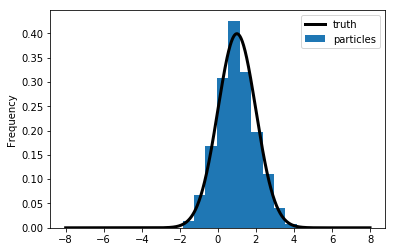
\includegraphics[width=.9\linewidth]{initialization.png}
\end{center}
\end{frame}

\begin{frame}[label={sec:orgbe8d29d}]{Forecasting \(s_1\)}
For each of the 1000 particles, we simulate from \(s_1^i = \rho s_0^i + \sigma_e e^i\) with \(e^i \sim N(0,1)\).
\begin{center}
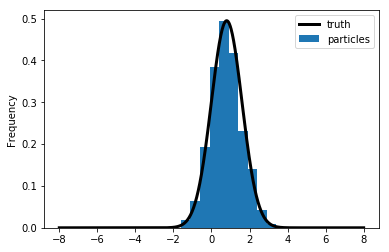
\includegraphics[width=.9\linewidth]{forecast.png}
\end{center}
\end{frame}


\begin{frame}[label={sec:org766d0c9}]{Updating \(s_1\)}
Now it's time to reweight the particles based on the how well they
actually predicted \(y_1\).
\\~\\~  
To predict \(y_1\), we simply multiply \(s_t^i\) by 2. 
\\~\\~  
How good is this prediction, let's think about in the context of ME.
\\~\\~  
\(y_1 = 0.2, \quad \sigma_u \in\{0.05, 0.3, 0.5\}\)
\\~\\~  
If the ME is very small, the only particles that make very accurate predictions are worthwhile.
\end{frame}
\begin{frame}[label={sec:orgc50614e}]{Predicting \(y_1\)}
\begin{center}
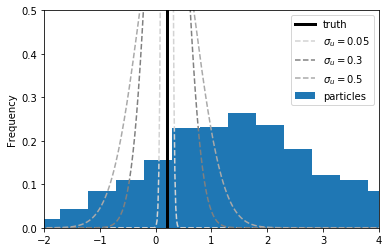
\includegraphics[width=.9\linewidth]{updated.png}
\end{center}
\end{frame}

\begin{frame}[label={sec:org5b4e2cd}]{Updated \(s_1, \sigma_u = 0.3\)}
\begin{center}
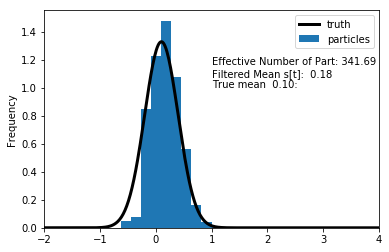
\includegraphics[width=.9\linewidth]{updated2.png}
\end{center}
\end{frame}

\begin{frame}[label={sec:org4ddba60}]{Updated \(s_1, \sigma_u = 0.5\)}
\begin{center}
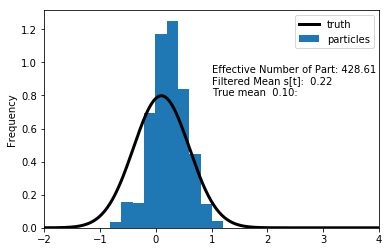
\includegraphics[width=.9\linewidth]{updated2big.png}
\end{center}
\end{frame}

\begin{frame}[label={sec:org0824345}]{Updated \(s_1, \sigma_u = 0.05\)}
\begin{center}
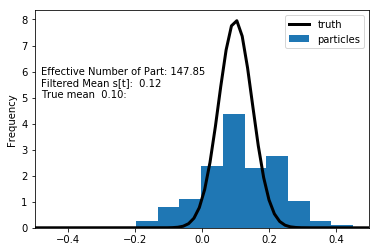
\includegraphics[width=.9\linewidth]{updated2small.png}
\end{center}
\end{frame}

\begin{frame}[label={sec:org496cfd4}]{Generic Particle Filter}
\begin{enumerate}
	\item {\bf Initialization.} Same as BS PF		
	\item {\bf Recursion.} For $t=1,\ldots,T$:
	\begin{enumerate}
		\item {\bf Forecasting $s_t$.} Draw $\tilde{s}_t^j$ from density $g_t(\tilde{s}_t|s_{t-1}^j,\theta)$
		and define 
		\be
		{\color{blue} \omega_t^j = \frac{p(\tilde{s}_t^j|s_{t-1}^j,\theta)}{g_t(\tilde{s}_t^j|s_{t-1}^j,\theta)}.}
		\label{eq_generalpfomega}
		\ee
		An approximation of $\mathbb{E}[h(s_t)|Y_{1:t-1},\theta]$ is given by
		\be
		\hat{h}_{t,M} = \frac{1}{M} \sum_{j=1}^M h(\tilde{s}_t^j) {\color{blue} \omega_t^j} W_{t-1}^j.
		\label{eq_generalpfhtt1}
		\ee
		\item {\bf Forecasting $y_t$.} Define the incremental weights
		$\tilde{w}^j_t = p(y_t|\tilde{s}^j_t,\theta) {\color{blue} \omega_t^j}$.

		The predictive density $p(y_t|Y_{1:t-1},\theta)$
		can be approximated by
		\be
		\hat{p}(y_t|Y_{1:t-1},\theta) = \frac{1}{M} \sum_{j=1}^M \tilde{w}^j_t W_{t-1}^j.
		\ee
		\item {\bf Updating.} Same as BS PF		
		\item {\bf Selection.} Same as BS PF		
	\end{enumerate}

\item \{\bf Likelihood Approximation.\} Same as BS PF		
\end{enumerate}
\end{frame}


\begin{frame}[label={sec:org2a6594e}]{Asymptotics}
\begin{itemize}
	\item The convergence results can be established recursively, starting from the assumption
	\begin{eqnarray*}
		\bar{h}_{t-1,M} &\stackrel{a.s.}{\longrightarrow}& \mathbb{E}[h(s_{t-1})|Y_{1:t-1}], \\
		\sqrt{M} \big( \bar{h}_{t-1,M} - \mathbb{E}[h(s_{t-1})|Y_{1:t-1}] \big) &\Longrightarrow& N \big( 0, \Omega_{t-1}(h) \big). \nonumber
	\end{eqnarray*}
	\item Forward iteration: draw $s_t$ from $g_t(s_t|s_{t-1}^j)= p(s_t|s_{t-1}^j)$.
	\item Decompose
	\begin{eqnarray}
	\lefteqn{\hat{h}_{t,M} - \mathbb{E}[h(s_t)|Y_{1:t-1}]}  \label{eq_pfdecomphtt1} \\
	&=& \frac{1}{M} \sum_{j=1}^M  \left( h(\tilde{s}_t^j) - \mathbb{E}_{p(\cdot|s_{t-1}^j)}[h] \right) W_{t-1}^j \nonumber \\
	& & + \frac{1}{M} \sum_{j=1}^M  \left( \mathbb{E}_{p(\cdot|s_{t-1}^j)}[h] W_{t-1}^j
	- \mathbb{E}[h(s_t)|Y_{1:t-1}] \right)  \nonumber \\
	&=& I + II, \nonumber
	\end{eqnarray}
	\item Both $I$ and $II$ converge to zero (and potentially satisfy CLT).
\end{itemize}
\end{frame}

\begin{frame}[label={sec:orgfaaf464}]{Asymptotics}
\begin{itemize}
	\item Updating step approximates
	\be\hspace{-0.4in}
	\mathbb{E}[h(s_t)|Y_{1:t}]
	= \frac{ \int h(s_t) p(y_t|s_t) p(s_t |Y_{1:t-1}) d s_t }{
		\int p(y_t|s_t) p(s_t |Y_{1:t-1}) d s_t }
	\approx \frac{ \frac{1}{M} \sum_{j=1}^M h(\tilde{s}_t^j) \tilde{w}_t^j W_{t-1}^j }{
		\frac{1}{M} \sum_{j=1}^M \tilde{w}_t^j W_{t-1}^j} 
	\ee
	\item Define the normalized incremental weights as
	\be
	v_t(s_t) = \frac{p(y_t|s_t)}{\int p(y_t|s_t) p(s_t|Y_{1:t-1}) ds_t}.
	\label{eq_pfincrweightv}
	\ee
	\item Under suitable regularity conditions, the Monte Carlo approximation satisfies a CLT of the
	form
	\begin{eqnarray}
	\lefteqn{\sqrt{M} \big( \tilde{h}_{t,M} - \mathbb{E}[h(s_t)|Y_{1:t}] \big) } \label{eq_pftildehclt} \\
	&\Longrightarrow& N \big( 0, \tilde{\Omega}_t(h) \big), \quad
	\tilde{\Omega}_t(h) = \hat{\Omega}_t \big( v_t(s_t) ( h(s_t) - \mathbb{E}[h(s_t)|Y_{1:t}] )\big). \nonumber
	\end{eqnarray}
	\item Distribution of particle weights matters for accuracy! $\Longrightarrow$ Resampling!
\end{itemize}
\end{frame}

\begin{frame}[label={sec:org1de14f3}]{Adapting the Generic PF}
\begin{itemize}
	\spitem Conditionally-optimal importance distribution:
		\[
		   g_t(\tilde{s}_t|s^j_{t-1}) = p(\tilde{s}_t|y_t,s_{t-1}^j).
		\]
		This is the posterior of $s_t$ given $s_{t-1}^j$. Typically infeasible, but a 
		good benchmark.
	\spitem Approximately conditionally-optimal distributions: from linearize version
		of DSGE model or approximate nonlinear filters.
	\spitem Conditionally-linear models: do Kalman filter updating on a subvector of $s_t$. Example:
	\begin{eqnarray*}
	y_t &=& \Psi_0(m_t) + \Psi_1(m_t) t + \Psi_2(m_t) s_t + u_t, \quad u_t \sim N(0,\Sigma_u), \label{eq_pfsslinearms} \\
	s_t &=& \Phi_0(m_t) + \Phi_1(m_t)s_{t-1} + \Phi_\epsilon(m_t) \epsilon_t, \quad \epsilon_t \sim N(0,\Sigma_\epsilon), \nonumber
	\end{eqnarray*}
	where $m_t$ follows a discrete Markov-switching process.
\end{itemize}
\end{frame}


\begin{frame}[label={sec:org3b38f33}]{More on Conditionally-Linear Models}
	\begin{itemize}
		\item State-space representation is linear conditional on $m_t$.
        \spitem Write
\be
p(m_{t},s_{t}|Y_{1:t}) = p(m_{t}|Y_{1:t})p(s_{t}|m_{t},Y_{1:t}),
\ee
where
\be
s_t|(m_t,Y_{1:t}) \sim N \big( \bar{s}_{t|t}(m_t), P_{t|t}(m_t) \big).
\ee
\item Vector of means $\bar{s}_{t|t}(m_t)$ and the covariance matrix
$P_{t|t}(m)_t$ are sufficient statistics for the conditional distribution of $s_t$.
\item Approximate $(m_t,s_t)|Y_{1:t}$ by $\{m_{t}^j,\bar{s}_{t|t}^j,P_{t|t}^j,W_t^j\}_{i=1}^N$. 
\item The swarm of particles approximates
\begin{eqnarray}
\lefteqn{\int h(m_{t},s_{t}) p(m_t,s_t,Y_{1:t}) d(m_t,s_t)} \\
&=& \int \left[ \int h(m_{t},s_{t}) p(s_{t}|m_{t},Y_{1:t}) d s_{t} \right] p(m_{t}|Y_{1:t}) dm_{t} \label{eq_pfraoapproxtt} \nonumber \\
&\approx&
\frac{1}{M} \sum_{j=1}^M \left[ \int h(m_{t}^j,s_{t}^j) p_N\big(s_t|\bar{s}_{t|t}^j,P_{t|t}^j \big) ds_t \right] W_t^j. \nonumber
\end{eqnarray}
\end{itemize}
\end{frame}

\begin{frame}[label={sec:orge4948b1}]{More on Conditionally-Linear Models}
	\begin{itemize}
		\item We used Rao-Blackwellization to reduce variance:
		\begin{eqnarray*}
\mathbb{V}[h(s_t,m_t)] &=& \mathbb{E} \big[ \mathbb{V}[h(s_t,m_t)|m_t] \big] + \mathbb{V} \big[ \mathbb{E}[h(s_t,m_t)|m_t] \big]\\& \ge& \mathbb{V} \big[ \mathbb{E}[h(s_t,m_t)|m_t] \big] 
\end{eqnarray*}
        \item To forecast the states in period $t$,
generate $\tilde{m}^j_t$ from  $g_t(\tilde{m}_t|m_{t-1}^j)$ and define:
\be
\omega_t^j = \frac{p(\tilde{m}_t^j|m_{t-1}^j)}{g_t(\tilde{m}_t^j|m_{t-1}^j)}.
\label{eq_generalpfomegacondlinear}
\ee
\item The Kalman filter
forecasting step can be used to compute:
\be
\begin{array}{lcl}
	\tilde{s}_{t|t-1}^j &=&  \Phi_0(\tilde{m}^j_t) + \Phi_1(\tilde{m}^j_t) s_{t-1}^j  \\
	P_{t|t-1}^j &=& \Phi_\epsilon(\tilde{m}^j_t) \Sigma_\epsilon(\tilde{m}^j_t) \Phi_\epsilon(\tilde{m}^j_t)' \\
	\tilde{y}_{t|t-1}^j &=& \Psi_0(\tilde{m}^j_t) + \Psi_1(\tilde{m}^j_t) t + \Psi_2(\tilde{m}^j_t) \tilde{s}_{t|t-1}^j \\ F_{t|t-1}^j &=& \Psi_2(\tilde{m}^j_t) P_{t|t-1}^j \Psi_2(\tilde{m}^j_t)' + \Sigma_u.
\end{array}
\label{eq_pfforeccondlinear}
\ee
\end{itemize}
\end{frame}



\begin{frame}[label={sec:org3bdadb5}]{More on Conditionally-Linear Models}
	\begin{itemize}
		
\item Then,
\begin{eqnarray}
\lefteqn{\int h(m_{t},s_{t}) p(m_t,s_t|Y_{1:t-1}) d(m_t,s_t)} \\
&=& \int \left[ \int h(m_{t},s_{t}) p(s_{t}|m_{t},Y_{1:t-1}) d s_{t} \right] p(m_{t}|Y_{1:t-1}) dm_{t} \label{eq_generalpfhtt1condlinear}  \nonumber \\
&\approx&\frac{1}{M} \sum_{j=1}^M \left[ \int h(m_{t}^j,s_{t}^j) p_N\big(s_t| \tilde{s}_{t|t-1}^j,P_{t|t-1}^j \big) ds_t \right] \omega_t^j W_{t-1}^j \nonumber
\end{eqnarray}
\item The likelihood approximation is based on the incremental weights
\be
\tilde{w}_t^j = p_N \big(y_t|\tilde{y}_{t|t-1}^j,F_{t|t-1}^j \big) \omega_t^j.
\label{eq_generalpfincrweightcondlinear}
\ee
\item Conditional on $\tilde{m}_t^j$ we can use the Kalman filter once more
to update the information about $s_t$ in view of the current observation $y_t$:
\be
\begin{array}{lcl}
	\tilde{s}_{t|t}^j &=& \tilde{s}_{t|t-1}^j + P_{t|t-1}^j \Psi_2(\tilde{m}^j_t)' \big( F_{t|t-1}^j \big)^{-1} (y_t - \bar{y}^j_{t|t-1}) \\
	\tilde{P}_{t|t}^j &=& P^j_{t|t-1} - P^j_{t|t-1} \Psi_2(\tilde{m}^j_t)'\big(F^j_{t|t-1} \big)^{-1} \Psi_2(\tilde{m}^j_t) P_{t|t-1}^j.
\end{array}
\label{eq_pfupdatecondlinear}
\ee
\end{itemize}
\end{frame}


\begin{frame}[label={sec:org879d9c1}]{Particle Filter For Conditionally Linear Models}
\begin{enumerate}
	\item {\bf Initialization.} 

	\item {\bf Recursion.} For $t=1,\ldots,T$:
	\begin{enumerate}
		\item {\bf Forecasting $s_t$.} Draw $\tilde{m}_t^j$ from density $g_t(\tilde{m}_t|m_{t-1}^j,\theta)$,
		calculate the importance weights $\omega_t^j$ in~(\ref{eq_generalpfomegacondlinear}),
		and compute $\tilde{s}_{t|t-1}^j$ and $P_{t|t-1}^j$ according to~(\ref{eq_pfforeccondlinear}).
		An approximation of $\mathbb{E}[h(s_t,m_t)|Y_{1:t-1},\theta]$ is given by~(\ref{eq_generalpfhtt1condlinear}).
		\item {\bf Forecasting $y_t$.} Compute the incremental weights $\tilde{w}_t^j$
		according to~(\ref{eq_generalpfincrweightcondlinear}).
		Approximate the predictive density $p(y_t|Y_{1:t-1},\theta)$
    by
		\be
		\hat{p}(y_t|Y_{1:t-1},\theta) = \frac{1}{M} \sum_{j=1}^M \tilde{w}^j_t W_{t-1}^j.
		\ee
		\item {\bf Updating.} Define the normalized weights
		\be
		\tilde{W}_t^j = \frac{\tilde{w}_t^j W_{t-1}^j}{\frac{1}{M} \sum_{j=1}^M \tilde{w}_t^j W_{t-1}^j}
		\ee
		and compute $\tilde{s}_{t|t}^j$ and $\tilde{P}_{t|t}^j$ according to~(\ref{eq_pfupdatecondlinear}). An approximation of $\mathbb{E}[h(m_{t},s_{t})|Y_{1:t},\theta]$ can be obtained
		from $\{\tilde{m}_t^j,\tilde{s}_{t|t}^j,\tilde{P}_{t|t}^j,\tilde{W}_t^j\}$.
		\item {\bf Selection.} 
	\end{enumerate}
\end{enumerate}
\end{frame}











\begin{frame}[label={sec:orgbe8d74f}]{Nonlinear and Partially Deterministic State Transitions}
\begin{itemize}
	\spitem Example:
	\[
	s_{1,t} = \Phi_1(s_{t-1},\epsilon_t), \quad s_{2,t} = \Phi_2(s_{t-1}), \quad \epsilon_t \sim N(0,1).
	\]
	\item Generic filter requires evaluation of $p(s_t|s_{t-1})$.
	\spitem Define $\varsigma_t = [s_t',\epsilon_t']'$ and add identity $\epsilon_t =
	\epsilon_t$ to state transition.
	\spitem Factorize the density
	$p(\varsigma_t|\varsigma_{t-1})$ as
	\[
	p(\varsigma_t|\varsigma_{t-1}) = p^\epsilon(\epsilon_t) p(s_{1,t}|s_{t-1},\epsilon_t) p(s_{2,t}|s_{t-1}).
	\]
	where $p(s_{1,t}|s_{t-1},\epsilon_t)$ and $p(s_{2,t}|s_{t-1})$ are
	pointmasses.
	\spitem Sample innovation
	$\epsilon_t$ from $g_t^\epsilon(\epsilon_t|s_{t-1})$.
	\spitem Then
	\[
	\omega_t^j = \frac{ p(\tilde{\varsigma}^j_t|\varsigma^j_{t-1}) }{g_t (\tilde{\varsigma}^j_t|\varsigma^j_{t-1})}
	= \frac{ p^\epsilon( \tilde{\epsilon}_t^j) p(\tilde{s}_{1,t}^j|s^j_{t-1},\tilde{\epsilon}^j_t) p(\tilde{s}^j_{2,t}|s^j_{t-1}) }
	{ g_t^\epsilon(\tilde{\epsilon}^j_t|s^j_{t-1}) p(\tilde{s}_{1,t}^j|s^j_{t-1},\tilde{\epsilon}^j_t) p(\tilde{s}^j_{2,t}|s^j_{t-1}) }
	= \frac{ p^\epsilon(\tilde{\epsilon}_t^j)}{g_t^\epsilon(\tilde{\epsilon}^j_t|s^j_{t-1})}.
	\label{eq_pfomegaepsilon}
	\]		
\end{itemize}
\end{frame}


\begin{frame}[label={sec:org3820dea}]{Degenerate Measurement Error Distributions}
\begin{itemize}
	\item  Our discussion of the conditionally-optimal
	importance distribution suggests that in the absence of measurement
	errors, one has to solve the system of equations
	\[ y_t = \Psi \big(
	\Phi( s_{t-1}^j,\tilde{\epsilon}_t^j) \big),
	\label{eq_pfepssystem}
	\]
	to determine $\tilde{\epsilon}_t^j$ as a function of $s_{t-1}^j$ and the current observation $y_t$. 
	\spitem Then define
	\[
	\omega_t^j = p^\epsilon(\tilde{\epsilon}_t^j) \quad \mbox{and} \quad
	\tilde{s}_t^j = \Phi( s_{t-1}^j,\tilde{\epsilon}_t^j).
	\]
	\item Difficulty: one has to find all solutions to a nonlinear system of equations.
	\spitem While resampling duplicates particles, the duplicated particles do not mutate, which
	can lead to a degeneracy. 
\end{itemize}
\end{frame}

\begin{frame}[label={sec:org332a46c}]{Next Steps}
\begin{itemize}
	\spitem We will now apply PFs to linearized DSGE models.
	\spitem This allows us to compare the Monte Carlo approximation to the ``truth.''
	\spitem Small-scale New Keynesian DSGE model
	\spitem Smets-Wouters model
\end{itemize}
\end{frame}

\begin{frame}[label={sec:orgcb8ee8f}]{Illustration 1: Small-Scale DSGE Model}
Parameter Values For Likelihood Evaluation
\begin{center}
	\begin{tabular}{lcclcc} \hline\hline
		Parameter & $\theta^{m}$ & $\theta^{l}$ & Parameter & $\theta^{m}$ & $\theta^{l}$  \\ \hline
		$\tau$               &  2.09 &  3.26 & $\kappa$             &  0.98 &  0.89 \\
		$\psi_1$             &  2.25 &  1.88 & $\psi_2$             &  0.65 &  0.53 \\
		$\rho_r$             &  0.81 &  0.76 & $\rho_g$             &  0.98 &  0.98 \\
		$\rho_z$             &  0.93 &  0.89 & $r^{(A)}$            &  0.34 &  0.19 \\
		$\pi^{(A)}$          &  3.16 &  3.29 & $\gamma^{(Q)}$       &  0.51 &  0.73 \\
		$\sigma_r$           &  0.19 &  0.20 & $\sigma_g$           &  0.65 &  0.58 \\
		$\sigma_z$           &  0.24 &  0.29 & $\ln p(Y|\theta)$    & -306.5 & -313.4 \\ \hline
	\end{tabular}
\end{center}
\end{frame}

\begin{frame}[label={sec:org4f2ef93}]{Likelihood Approximation}
\begin{center}
	\begin{tabular}{c}
		$\ln \hat{p}(y_t|Y_{1:t-1},\theta^m)$ vs. $\ln p(y_t|Y_{1:t-1},\theta^m)$ \\
		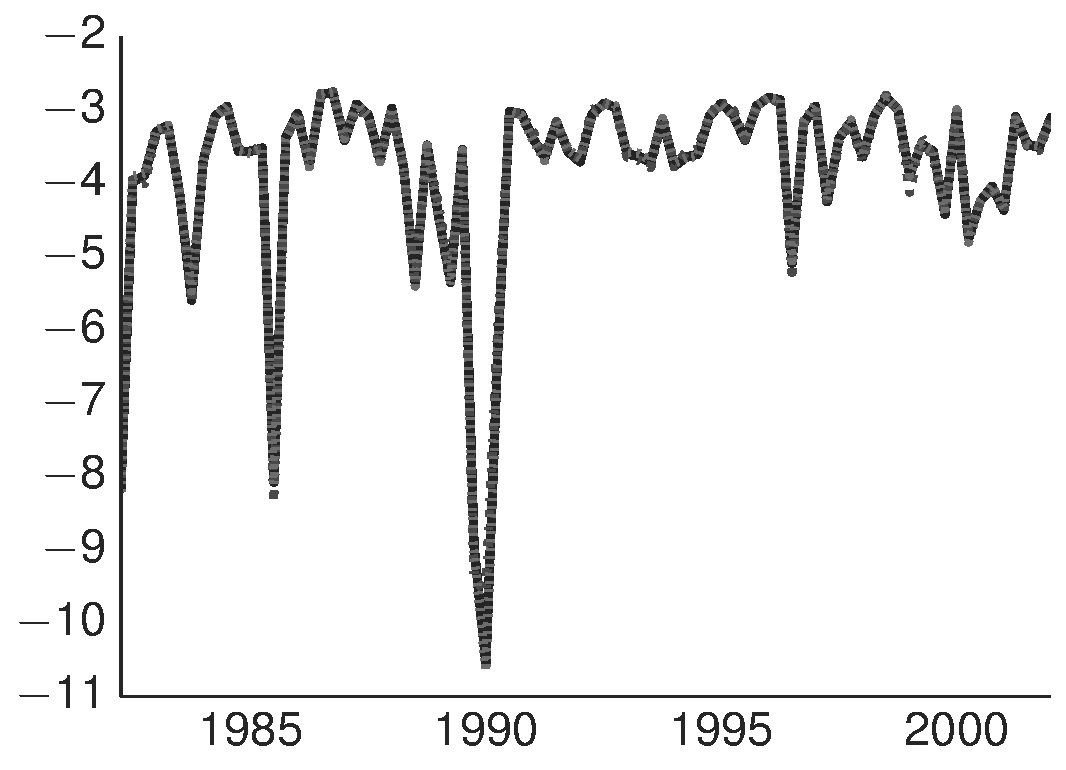
\includegraphics[width=3.2in]{dsge1_me_paramax_lnpy.pdf} 
	\end{tabular}
\end{center}
\uline{Notes}: The results depicted in the figure are based on a single run
of the bootstrap PF (dashed, \(M=40,000\)), the conditionally-optimal PF (dotted, \(M=400\)), and the Kalman filter (solid).
\end{frame}


\begin{frame}[label={sec:orgc4b6f0a}]{Filtered State}
\begin{center}
	\begin{tabular}{c}
		$\widehat{\mathbb{E}}[\hat{g}_t|Y_{1:t},\theta^m]$ vs. $\mathbb{E}[\hat{g}_t|Y_{1:t},\theta^m]$\\
		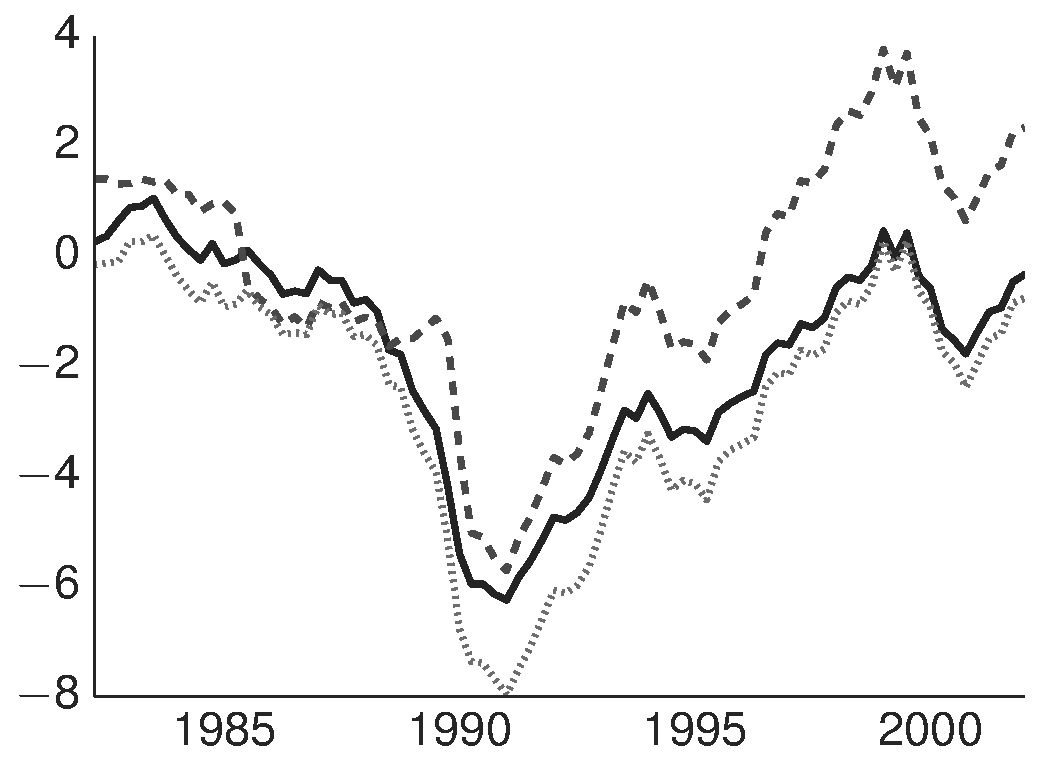
\includegraphics[width=3.2in]{dsge1_me_paramax_ghat.pdf}
	\end{tabular}
\end{center}
\uline{Notes}: The results depicted in the figure are based on a single run
of the bootstrap PF (dashed, \(M=40,000\)), the conditionally-optimal PF (dotted, \(M=400\)), and the Kalman filter (solid).
\end{frame}

\begin{frame}[label={sec:orgbad312c}]{Distribution of Log-Likelihood Approximation Errors\}}
\begin{center}
	\begin{tabular}{c}
		Bootstrap PF: $\theta^m$ vs. $\theta^l$ \\
		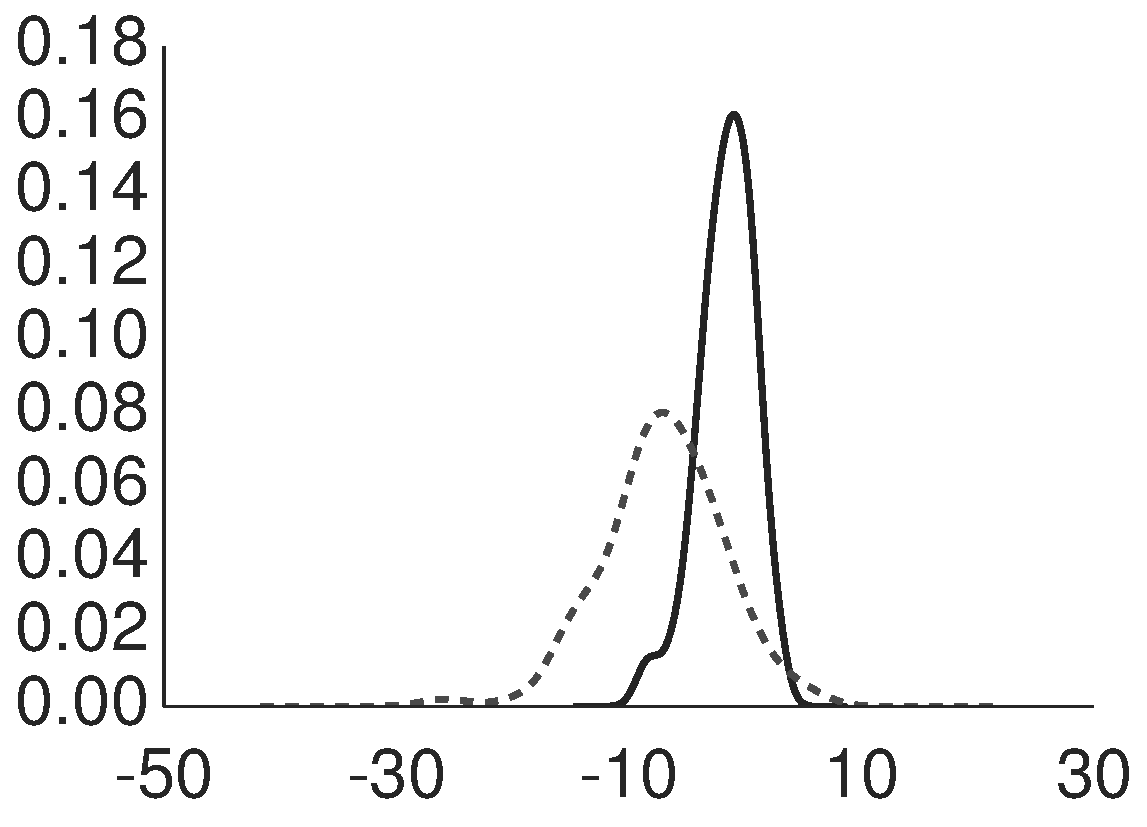
\includegraphics[width=3in]{dsge1_me_bootstrap_lnlhbias.pdf}
	\end{tabular}
\end{center}
\uline{Notes}: Density estimate of \(\hat{\Delta}_1 = \ln \hat{p}(Y_{1:T}|\theta)- \ln p(Y_{1:T}|\theta)\)
based on \(N_{run}=100\) runs of the PF. Solid line is \(\theta = \theta^m\); dashed line is \(\theta = \theta^l\) 
(\(M=40,000\)).
\end{frame}

\begin{frame}[label={sec:orgff59350}]{Distribution of Log-Likelihood Approximation Errors\}}
\begin{center}
	\begin{tabular}{c}
		$\theta^m$: Bootstrap vs. Cond. Opt. PF \\
		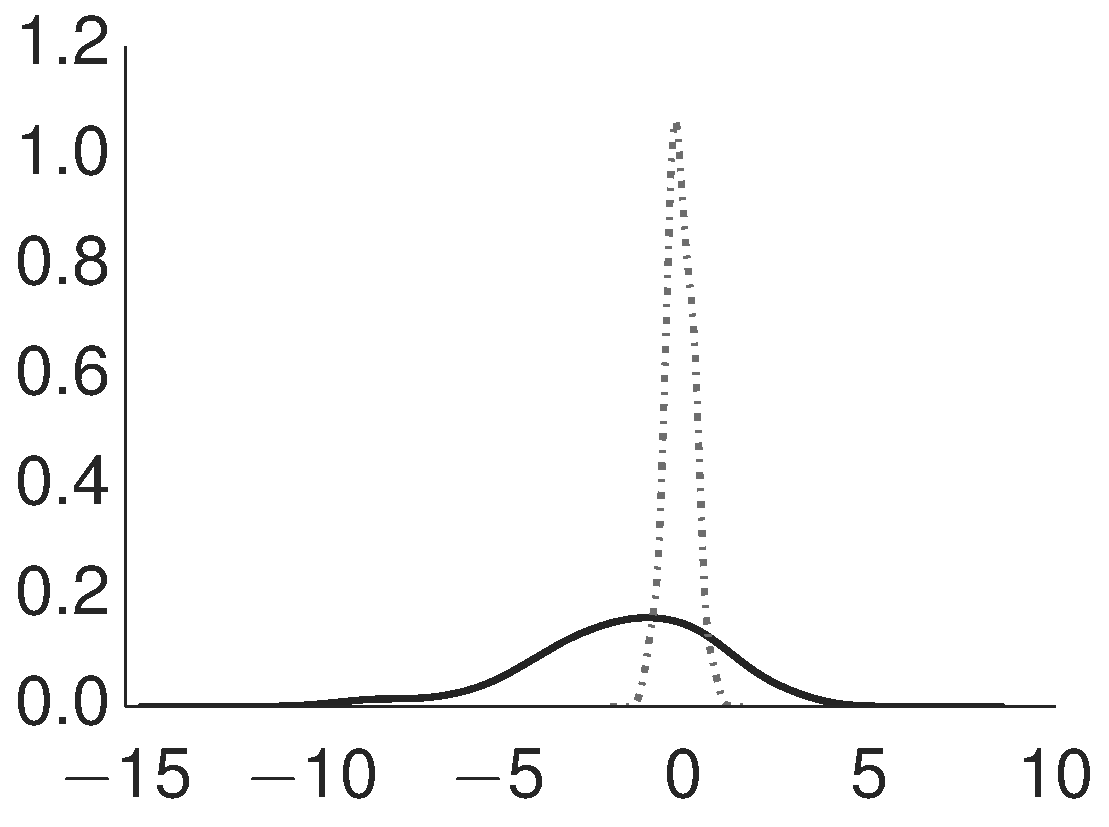
\includegraphics[width=3in]{dsge1_me_paramax_lnlhbias.pdf} \\
	\end{tabular}
\end{center}
\uline{Notes}: Density estimate of \(\hat{\Delta}_1 = \ln \hat{p}(Y_{1:T}|\theta)- \ln p(Y_{1:T}|\theta)\)
based on \(N_{run}=100\) runs of the PF. Solid line is bootstrap particle filter
(\(M=40,000\)); dotted line is conditionally optimal particle filter
(\(M=400\)).
\end{frame}

\begin{frame}[label={sec:org53a88e0}]{Summary Statistics for Particle Filters}
\begin{center}
	\begin{tabular}{lrrr} \\ \hline \hline
		& Bootstrap & Cond. Opt. & Auxiliary \\ \hline
		Number of Particles $M$ & 40,000 & 400 & 40,000 \\
		Number of Repetitions   & 100 & 100 & 100 \\ \hline
		\multicolumn{4}{c}{High Posterior Density: $\theta = \theta^m$} \\ \hline
		Bias $\hat{\Delta}_1$ & -1.39 & -0.10 & -2.83 \\
		StdD $\hat{\Delta}_1$ &  2.03 &  0.37 &  1.87 \\
		Bias $\hat{\Delta}_2$ &  0.32 & -0.03 & -0.74 \\ \hline
		\multicolumn{4}{c}{Low Posterior Density: $\theta = \theta^l$} \\ \hline
		Bias $\hat{\Delta}_1$ & -7.01 & -0.11 & -6.44 \\
		StdD $\hat{\Delta}_1$ &  4.68 &  0.44 &  4.19 \\
		Bias $\hat{\Delta}_2$ & -0.70 & -0.02 & -0.50 \\ \hline
	\end{tabular}
\end{center}
\uline{Notes}: \(\hat{\Delta}_1 = \ln \hat{p}(Y_{1:T}|\theta) - \ln p(Y_{1:T}|\theta)\)
and \(\hat{\Delta}_2 = \exp[ \ln \hat{p}(Y_{1:T}|\theta) - \ln
	p(Y_{1:T}|\theta) ] - 1\). Results
are based on \(N_{run}=100\) runs of the particle filters.
\end{frame}


\begin{frame}[label={sec:org4563894}]{Great Recession and Beyond}
\begin{center}
	\begin{tabular}{c}
		Mean of Log-likelihood Increments $\ln \hat{p}(y_t|Y_{1:t-1},\theta^m)$ \\
		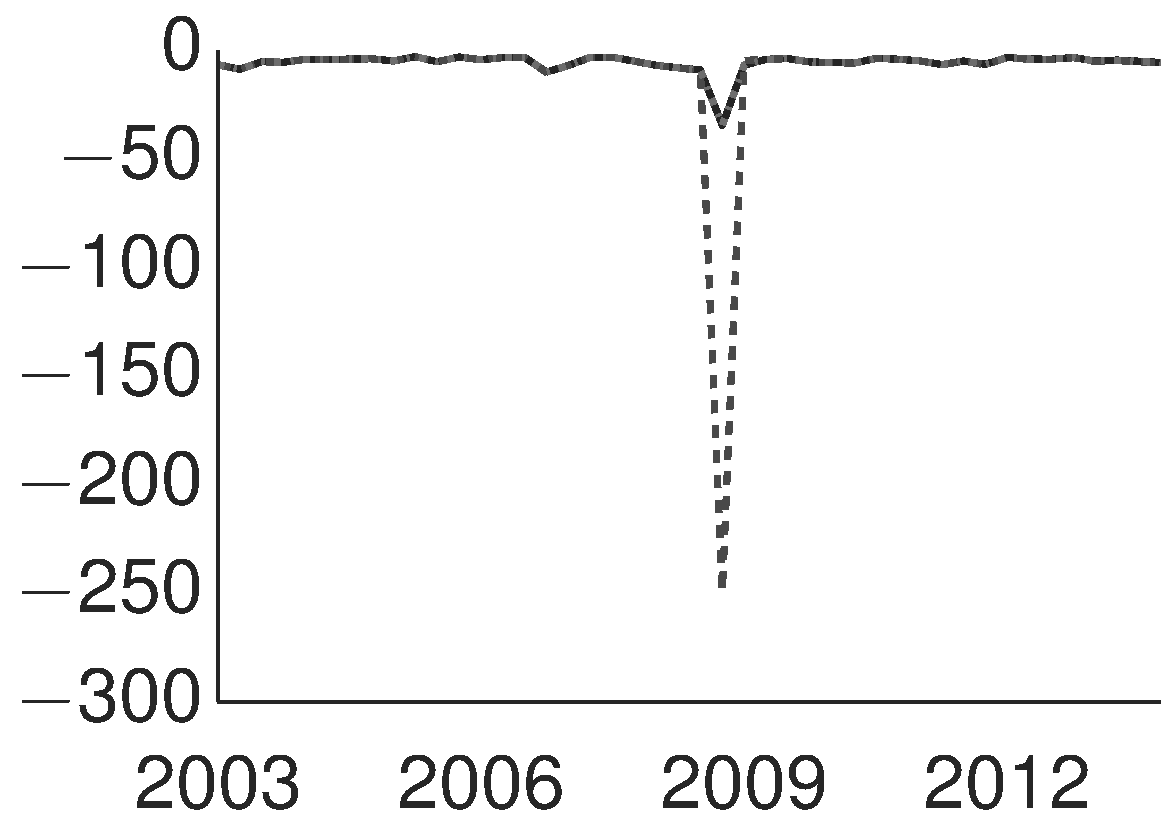
\includegraphics[width=3in]{dsge1_me_great_recession_lnpy.pdf} 
	\end{tabular}
\end{center}
\uline{Notes}: Solid lines represent results from Kalman
filter. Dashed lines correspond to bootstrap particle filter
(\(M=40,000\)) and dotted lines correspond to
conditionally-optimal particle filter (\(M=400\)). Results are
based on \(N_{run}=100\) runs of the filters.
\end{frame}


\begin{frame}[label={sec:org4a1ae59}]{Great Recession and Beyond}
\begin{center}
	\begin{tabular}{c}
    Mean of Log-likelihood Increments $\ln \hat{p}(y_t|Y_{1:t-1},\theta^m)$ \\
		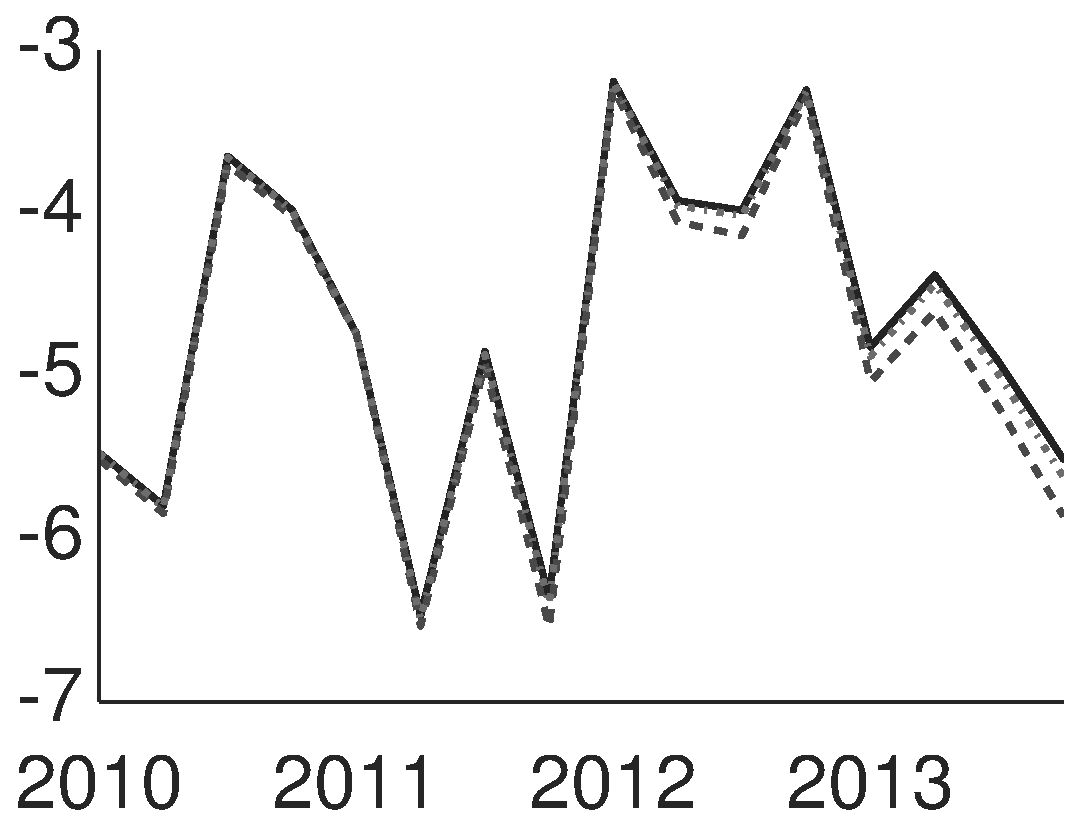
\includegraphics[width=2.9in]{dsge1_me_post_great_recession_lnpy.pdf} 
	\end{tabular}
\end{center}
\uline{Notes}: Solid lines represent results from Kalman
filter. Dashed lines correspond to bootstrap particle filter
(\(M=40,000\)) and dotted lines correspond to
conditionally-optimal particle filter (\(M=400\)). Results are
based on \(N_{run}=100\) runs of the filters.
\end{frame}

\begin{frame}[label={sec:org4284cfa}]{Great Recession and Beyond}
\begin{center}
	\begin{tabular}{c}
    Log Standard Dev of Log-Likelihood Increments \\
    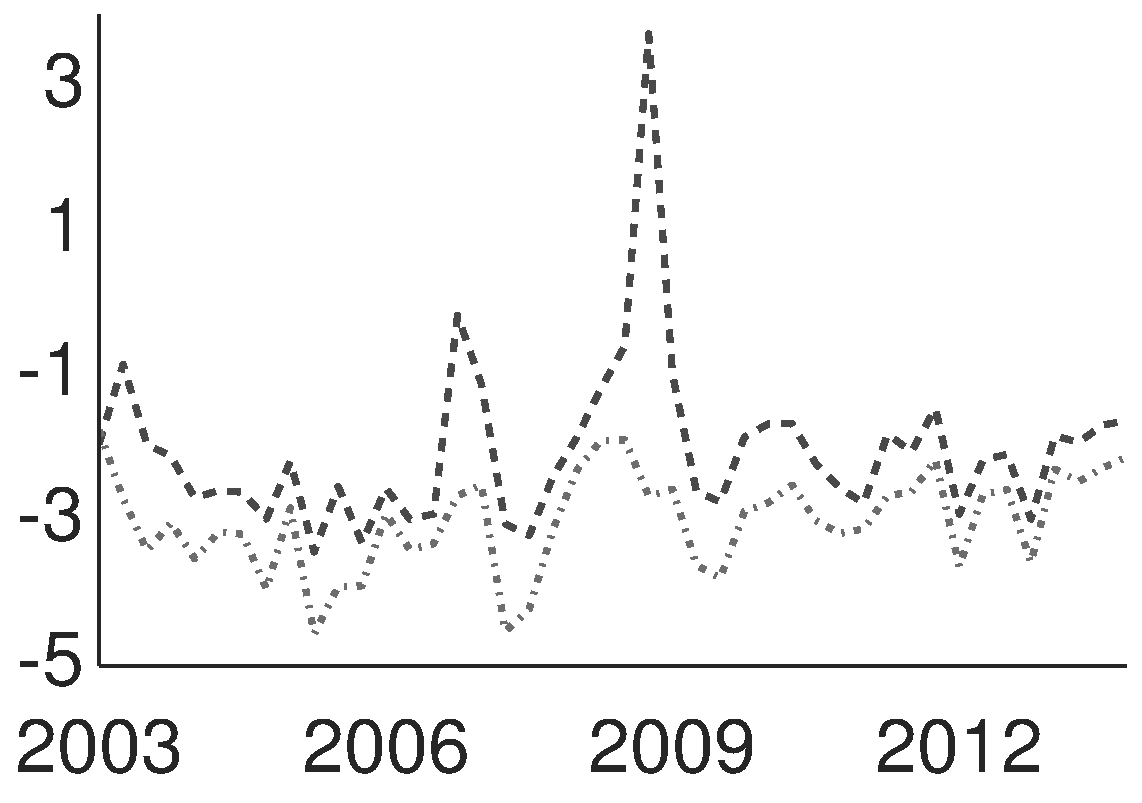
\includegraphics[width=3in]{dsge1_me_great_recession_lnpy_lnstd.pdf} 
\end{tabular}
\end{center}
\uline{Notes}: Solid lines represent results from Kalman
filter. Dashed lines correspond to bootstrap particle filter
(\(M=40,000\)) and dotted lines correspond to
conditionally-optimal particle filter (\(M=400\)). Results are
based on \(N_{run}=100\) runs of the filters.
\end{frame}

\begin{frame}[label={sec:orga89a475}]{SW Model: Distr. of Log-Likelihood Approximation Errors}
\begin{center}
	\begin{tabular}{c}
		BS ($M=40,000$) versus CO ($M=4,000$) \\
		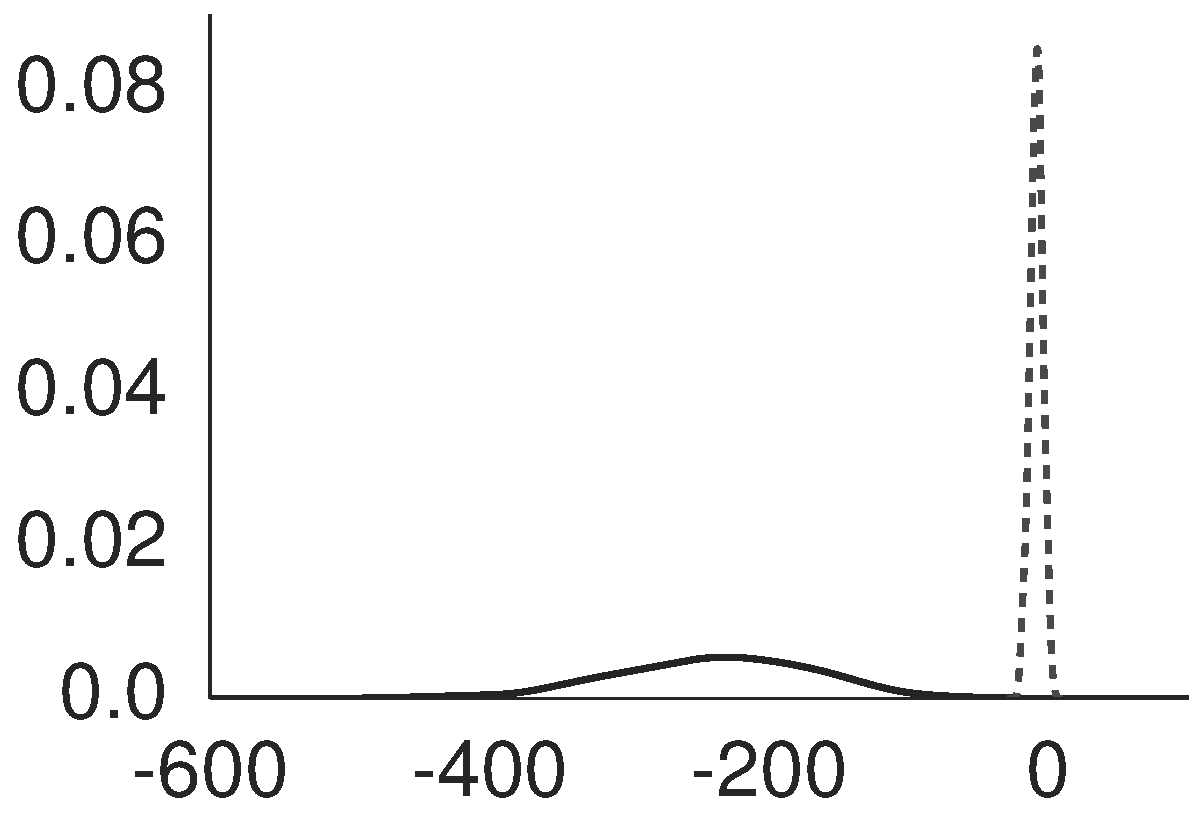
\includegraphics[width=3in]{sw_me_paramax_lnlhbias.pdf}
	\end{tabular}
\end{center}
\uline{Notes}: Density estimates of \(\hat{\Delta}_1 = \ln \hat{p}(Y|\theta)- \ln p(Y|\theta)\) based on \(N_{run}=100\).
Solid densities summarize results for the bootstrap (BS) particle filter;
dashed densities summarize results for the conditionally-optimal (CO) particle filter.
\end{frame}

\begin{frame}[label={sec:org171426d}]{SW Model: Distr. of Log-Likelihood Approximation Errors}
\begin{center}
	\begin{tabular}{c}
		BS ($M=400,000$) versus CO ($M=4,000$) \\
		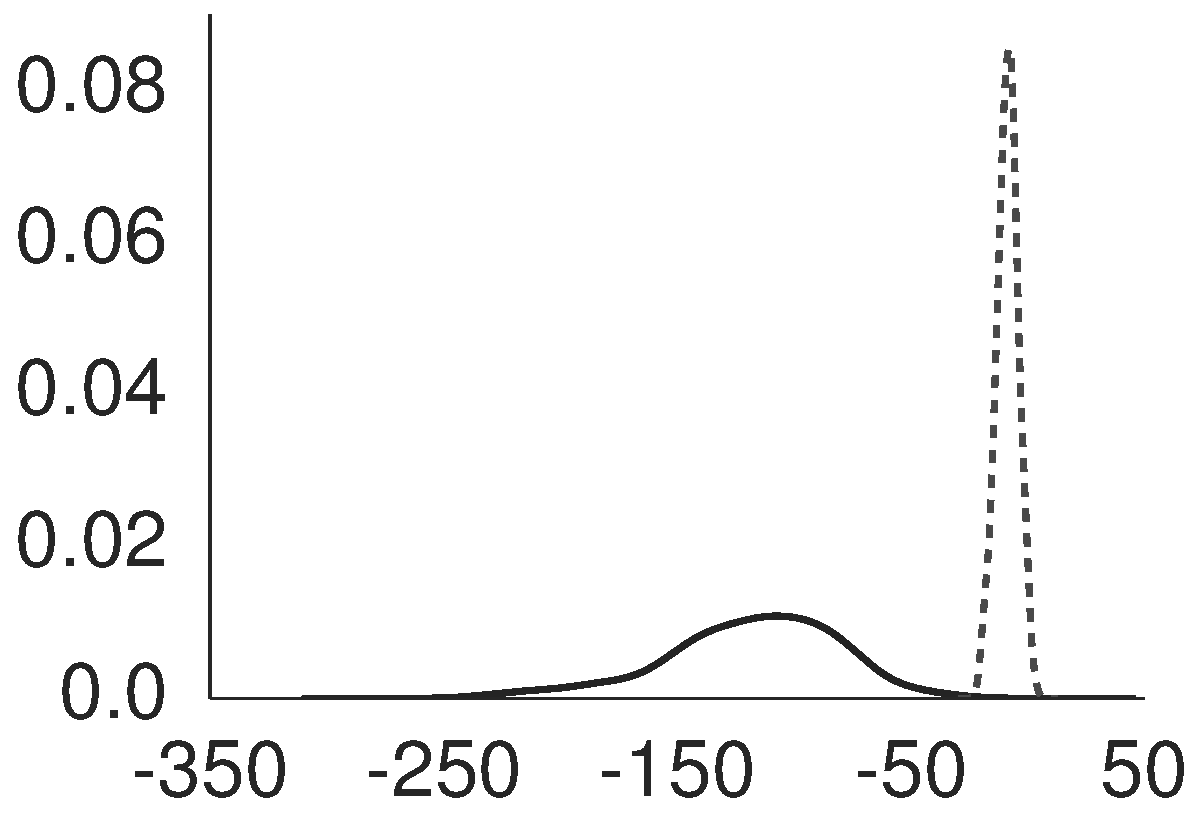
\includegraphics[width=3in]{sw_me_paramax_bs_lnlhbias.pdf}
	\end{tabular}
\end{center}
\uline{Notes}: Density estimates of \(\hat{\Delta}_1 = \ln \hat{p}(Y|\theta)- \ln p(Y|\theta)\) based on \(N_{run}=100\).
Solid densities summarize results for the bootstrap (BS) particle filter;
dashed densities summarize results for the conditionally-optimal (CO) particle filter.
\end{frame}


\begin{frame}[label={sec:org709dc80}]{SW Model: Summary Statistics for Particle Filters}
\begin{center}
	\begin{tabular}{lrrrr} \\ \hline \hline
		& \multicolumn{2}{c}{Bootstrap} & \multicolumn{2}{c}{Cond. Opt.} \\ \hline
		Number of Particles $M$ & 40,000 & 400,000 & 4,000 & 40,000 \\
		Number of Repetitions   & 100 & 100 & 100 & 100 \\ \hline
		\multicolumn{5}{c}{High Posterior Density: $\theta = \theta^m$} \\ \hline
		Bias $\hat{\Delta}_1$ & -238.49 & -118.20 &   -8.55 &   -2.88 \\
		StdD $\hat{\Delta}_1$ &   68.28 &   35.69 &    4.43 &    2.49 \\
		Bias $\hat{\Delta}_2$ &   -1.00 &   -1.00 &   -0.87 &   -0.41 \\ \hline
		\multicolumn{5}{c}{Low Posterior Density: $\theta = \theta^l$} \\ \hline
		Bias $\hat{\Delta}_1$ & -253.89 & -128.13 &  -11.48 &   -4.91 \\
		StdD $\hat{\Delta}_1$ &   65.57 &   41.25 &    4.98 &    2.75 \\
		Bias $\hat{\Delta}_2$ &   -1.00 &   -1.00 &   -0.97 &   -0.64 \\ \hline
	\end{tabular}
\end{center}
\uline{Notes}: \(\hat{\Delta}_1 = \ln \hat{p}(Y_{1:T}|\theta) - \ln p(Y_{1:T}|\theta)\)
and \(\hat{\Delta}_2 = \exp[ \ln \hat{p}(Y_{1:T}|\theta) - \ln
	p(Y_{1:T}|\theta) ] - 1\). Results are based on \(N_{run}=100\). 
\end{frame}

\section{Tempered Particle Filtering}
\label{sec:org615ec00}

\begin{frame}[label={sec:orgecf662b}]{Tempered Particle Filter}
\begin{itemize}
\item Use sequence of distributions between the forecast and updated state distributions.
\end{itemize}
\\~\\~     
\begin{itemize}
\item Candidates? Well, \emph{the PF will work arbitrarily well when \(\Sigma_{u}\rightarrow\infty\).}
\end{itemize}
\\~\\~     
\begin{itemize}
\item \alert{Reduce measurement error variance from an inflated initial level}
\(\Sigma_u(\theta)/{\color{blue}\phi_1}\) to the nominal level \(\Sigma_u(\theta)\).
\end{itemize}
\end{frame}

\begin{frame}[label={sec:orgf058353}]{The Key Idea}
\begin{itemize}
\item Define
\begin{eqnarray*} p_n(y_t|s_t,\theta) &\propto& {\color{blue}\phi_n^{d/2}}
|\Sigma_u(\theta)|^{-1/2}\exp \bigg\{ - \frac{1}{2} (y_t - \Psi(s_t,t;\theta))' \\
&& \times {\color{blue}\phi_n} \Sigma_u^{-1}(\theta)(y_t - \Psi(s_t,t;\theta)) \bigg\},
\end{eqnarray*}
where:
\[
      {\color{blue} \phi_1 < \phi_2 < \ldots < \phi_{N_\phi} = 1}.
      \]
\item \alert{Bridge posteriors given \(s_{t-1}\):}
\[
      p_n(s_t|y_t,s_{t-1},\theta)
        \propto p_n(y_t|s_t,\theta) p(s_t|s_{t-1},\theta).
      \]
\item \alert{bridge posteriors given \(Y_{1:t-1}\):}
\[
      p_n(s_t|Y_{1:t})= \int p_n(s_t|y_t,s_{t-1},\theta) p(s_{t-1}|Y_{1:t-1}) ds_{t-1}.
      \]
\end{itemize}
\end{frame}

\begin{frame}[label={sec:orgbb1c5b1}]{Algorithm Overview}
\begin{itemize}
\item For each \(t\) we start with the BS-PF iteration by simulating the state-transition equation forward.
\\~\\~
\item Incremental weights are obtained based on \alert{inflated measurement error variance} \(\Sigma_u/{\color{blue}\phi_1}\).
\\~\\~
\item \emph{Then we start the tempering iterations}\ldots{}
\\~\\~
\item After the tempering iterations are completed we proceed to \(t+1\)\ldots{}
\end{itemize}
\end{frame}

\begin{frame}[label={sec:org56e9663}]{Overview\}}
\begin{itemize}
\item If \(N_{\phi} = 1\), this collapses to the Bootstrap particle filter.
\\~\\~
\item For each time period \(t\), we embed a ``static'' SMC sampler used for parameter estimation
Iterate over \(n=1,\ldots,N_\phi\):
\begin{itemize}
\item \alert{Correction step}:  change particle weights (importance sampling)
\item \alert{Selection step}: equalize particle weights (resampling of particles)
\item \alert{Mutation step}: change particle values (based on Markov transition kernel generated with Metropolis-Hastings algorithm)
\item Each step approximates the same \(\int h(s_t) p_n(s_{t}|Y_{1:t},\theta) ds_t\).
\end{itemize}
\end{itemize}
\end{frame}

\begin{frame}[label={sec:orgff328e2}]{An Illustration: \(p_n(s_t|Y_{1:t})\), \(n=1,\ldots,N_\phi\).}
\begin{center}
	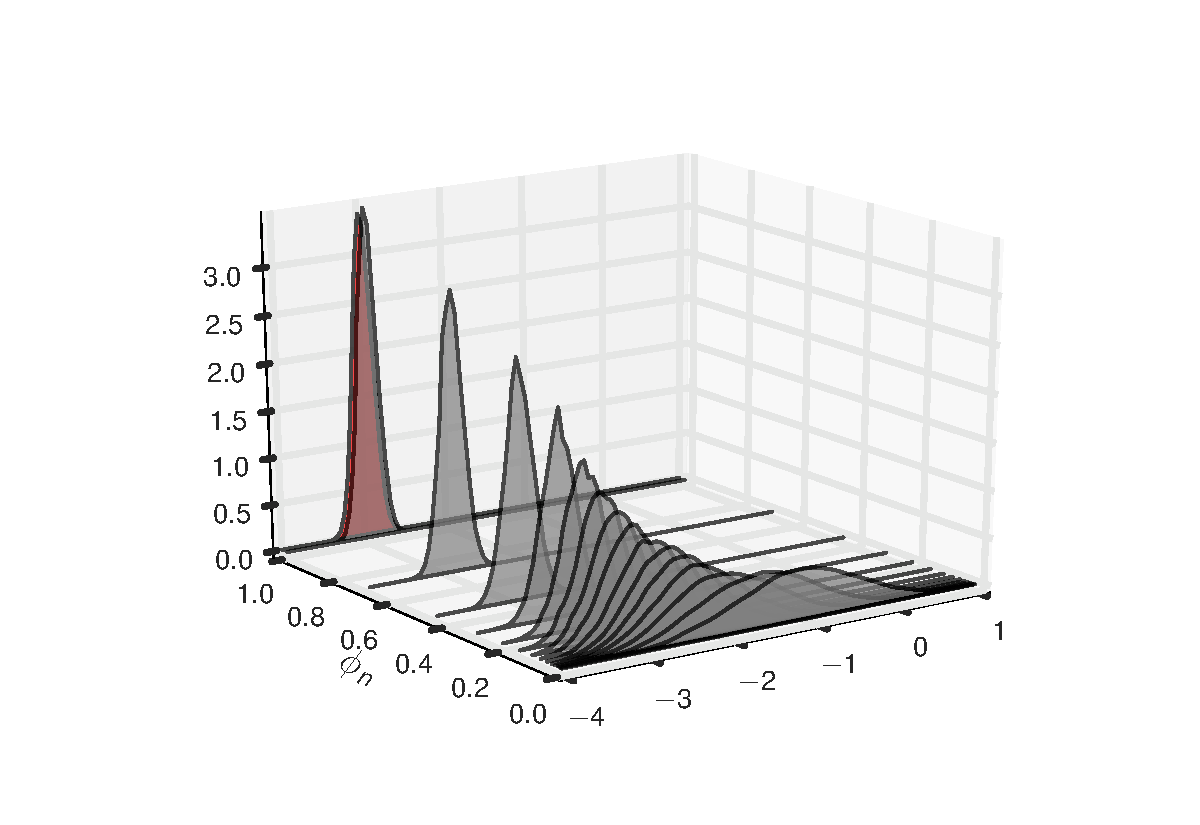
\includegraphics[width=4in]{phi_evolution.pdf}
\end{center}
\end{frame}


\begin{frame}[label={sec:org4f58cef}]{Choice of \(\phi_n\)}
\begin{itemize}
\item Based on Geweke and Frischknecht (2014).
\\~\\~
\item Express post-correction inefficiency ratio as
\[
             \mbox{InEff}(\phi_n)
             =  \frac{\frac{1}{M} \sum_{j=1}^M \exp [ -2(\phi_n-\phi_{n-1}) e_{j,t}] }{ \left(\frac{1}{M} \sum_{j=1}^M  \exp [ -(\phi_n-\phi_{n-1}) e_{j,t}] \right)^2}
     \]
where
\[
       e_{j,t} = \frac{1}{2} (y_t - \Psi(s_t^{j,n-1},t;\theta))' \Sigma_u^{-1}(y_t -
       \Psi(s_t^{j,n-1},t;\theta)).
     \]
\\~\\~
\item Pick target ratio \(r^*\) and solve equation \(\mbox{InEff}(\phi_n^*) = r^*\) for \(\phi_n^*\).
\end{itemize}

\end{frame}
\end{frame}



\begin{frame}[label={sec:org1ac0a48}]{Small-Scale Model: PF Summary Statistics}
\begin{center}
	\begin{tabular}{l@{\hspace{1cm}}r@{\hspace{1cm}}rrrr}												    \\ \hline \hline
		& BSPF	 & \multicolumn{4}{c}{TPF} \\ \hline
		Number of Particles $M$		 & 40k & 4k	    & 4k	  & 40k		& 40k	       \\
		Target Ineff. Ratio $r^*$	     &	   & 2		  & 3		   & 2		    & 3		   \\ \hline
		\multicolumn{6}{c}{High Posterior Density: $\theta = \theta^m$}						      \\ \hline
		Bias		& -1.4 & -0.9 & -1.5 & -0.3 & -.05     \\
		StdD		& 1.9  & 1.4  & 1.7  & 0.4  & 0.6	\\
		$T^{-1}\sum_{t=1}^{T}N_{\phi,t}$      & 1.0  & 4.3  & 3.2  & 4.3 & 3.2			  \\
		Average Run Time (s)		 & 0.8	& 0.4 & 0.3 & 4.0 & 3.3	     \\ \hline
		\multicolumn{6}{c}{Low Posterior Density: $\theta = \theta^l$}						      \\ \hline
		Bias		 & -6.5 & -2.1 & -3.1 & -0.3  & -0.6		      \\
		StdD		 & 5.3	& 2.1  & 2.6  & 0.8   & 1.0		       \\
		$T^{-1}\sum_{t=1}^{T}N_{\phi,t}$       & 1.0  & 4.4 & 3.3     & 4.4 & 3.3	       \\
		Average Run Time (s)		 & 1.6 & 0.4 & 0.3 & 3.7     & 2.9		      \\ \hline
	\end{tabular}
\end{center}
\end{frame}



\begin{frame}[label={sec:orga41a2c8}]{Embedding PF Likelihoods into Posterior Samplers}
\begin{itemize}
\item Likelihood functions for nonlinear DSGE models can be approximated by the PF.
\\~\\~
\item We will now embed the likelihood approximation into a posterior sampler:
PFMH Algorithm (a special case of PMCMC).
\\~\\~
\item The book also discusses \(SMC^2\).
\end{itemize}
\end{frame}



\begin{frame}[label={sec:org8a4c273}]{Embedding PF Likelihoods into Posterior Samplers\}}
\begin{itemize}
\item \(\{ p(Y|\theta), p(\theta|Y), p(Y) \}\), which are related according to:
\end{itemize}
\[
   p(\theta|Y) = \frac{p(Y|\theta) p(\theta)}{p(Y)} , \quad p(Y) = \int p(Y|\theta) p(\theta) d\theta
   \]
\begin{itemize}
\item \(\{ \hat{p}(Y|\theta), \hat{p}(\theta|Y), \hat{p}(Y) \}\), which are related according to:
\end{itemize}
\[
   \hat{p}(\theta|Y) = \frac{\hat{p}(Y|\theta) p(\theta)}{\hat{p}(Y)} , \quad \hat{p}(Y) = \int \hat{p}(Y|\theta) p(\theta) d\theta.
   \]
\begin{itemize}
\item Surprising result (Andrieu, Docet, and Holenstein, 2010): under certain conditions we can replace \(p(Y|\theta)\) by \(\hat{p}(Y|\theta)\) and still obtain draws from \(p(\theta|Y)\).
\end{itemize}
\end{frame}


\begin{frame}[label={sec:org7251c95}]{PFMH Algorithm}
For \(i=1\) to \(N\):
\begin{enumerate}
\item Draw \(\vartheta\) from a density \(q(\vartheta|\theta^{i-1})\).
\\~\\~
\item Set \(\theta^i = \vartheta\) with probability
\[
   \alpha(\vartheta | \theta^{i-1} ) = \min \left\{ 1, \;
   \frac{ \hat{p}(Y| \vartheta )p(\vartheta) / q(\vartheta | \theta^{i-1}) }{
           \hat{p}(Y|\theta^{i-1}) p(\theta^{i-1})	 / q(\theta^{i-1} | \vartheta) } \right\}
   \]
and \(\theta^{i} = \theta^{i-1}\) otherwise. The likelihood approximation \(\hat{p}(Y|\vartheta)\) is computed using a particle filter.
\end{enumerate}
\end{frame}

\begin{frame}[label={sec:orga320eec}]{Why Does the PFMH Work?}
\begin{itemize}
\item At each iteration the filter generates draws \(\tilde{s}_t^j\) from the proposal distribution \(g_t(\cdot|s_{t-1}^j)\).
\\~\\~
\item Let \(\tilde{S}_t = \big( \tilde{s}_t^1,\ldots,\tilde{s}_t^M \big)'\) and denote the entire sequence of draws by \(\tilde{S}_{1:T}^{1:M}\).
\\~\\~
\item Selection step: define a random variable \(A_t^j\) that contains this ancestry information.  For instance, suppose that during the resampling particle \(j=1\) was assigned the value \(\tilde{s}_t^{10}\) then \(A_t^1=10\). Let \(A_t = \big( A_t^1, \ldots, A_t^N \big)\) and use \(A_{1:T}\) to denote the sequence of \(A_t\)'s.
\\~\\~
\item PFMH operates on an enlarged probability space: \(\theta\), \(\tilde{S}_{1:T}\) and \(A_{1:T}\).
\end{itemize}
\end{frame}

\begin{frame}[label={sec:org025c825}]{Why Does the PFMH Work?}
\begin{itemize}
\item Use \(U_{1:T}\) to denote random vectors for \(\tilde{S}_{1:T}\) and \(A_{1:T}\). \(U_{1:T}\) is an array of \(iid\) uniform random numbers.
\\~\\~
\item The transformation of \(U_{1:T}\) into \((\tilde{S}_{1:T},A_{1:T})\) typically depends on \(\theta\) and \(Y_{1:T}\), because the proposal distribution \(g_t(\tilde{s}_t|s_{t-1}^j)\) depends both on the current observation \(y_t\) as well as the parameter vector \(\theta\).
\\~\\~
\item E.g., implementation of conditionally-optimal PF  requires sampling from a \(N(\bar{s}_{t|t}^j,P_{t|t})\) distribution for each particle \(j\). Can be done using a prob integral transform of uniform random variables.
\\~\\~
\item We can express the particle filter approximation of the likelihood function as
\[
	\hat{p}(Y_{1:T}|\theta) = g(Y_{1:T}|\theta,U_{1:T}).
	\]
where
\[
	U_{1:T} \sim p(U_{1:T}) = \prod_{t=1}^T p(U_t).
	\]
\end{itemize}
\end{frame}


\begin{frame}[label={sec:org9fc9bb4}]{Why Does the PFMH Work?}
\begin{itemize}
\item Define the joint distribution
\[
     p_g\big( Y_{1:T},\theta,U_{1:T} \big) = g(Y_{1:T}|\theta,U_{1:T}) p\big(U_{1:T} \big) p(\theta).
     \]
\item The PFMH algorithm samples from the joint posterior
 \[
      p_g\big( \theta, U_{1:T} | Y_{1:T} \big) \propto g(Y|\theta,U_{1:T}) p\big(U_{1:T} \big) p(\theta)
      \]
 and discards the draws of \(\big( U_{1:T} \big)\).
\\~\\~
\item For this procedure to be valid, it needs to be the case that PF approximation is unbiased:
\[
     \mathbb{E}[\hat{p}(Y_{1:T}|\theta)]
     = \int g(Y_{1:T}|\theta,U_{1:T})p\big(U_{1:T} \big) d\theta
     = p(Y_{1:T}|\theta).
     \]
\end{itemize}
\end{frame}

\begin{frame}[label={sec:org2f6023b}]{Why Does the PFMH Work?}
\begin{itemize}
\item We can express acceptance probability directly in terms of \(\hat{p}(Y_{1:T}|\theta)\).
\item Need to generate a proposed draw for both \(\theta\) and \(U_{1:T}\): \(\vartheta\) and \(U_{1:T}^*\).
\item The proposal distribution for \((\vartheta,U_{1:T}^*)\) in the MH algorithm is given by \(q(\vartheta|\theta^{(i-1)}) p(U_{1:T}^*)\).
\item No need to keep track of the draws \((U_{1:T}^*)\).
\item MH acceptance probability:
\begin{eqnarray*}
	\alpha(\vartheta|\theta^{i-1})
	&=&
	\min \; \left\{ 1,
	\frac{ \frac{ g(Y|\vartheta,U^*)p(U^*) p(\vartheta)}{ q(\vartheta|\theta^{(i-1)}) p(U^*) } }{
	      \frac{ g(Y|\theta^{(i-1)},U^{(i-1)})p(U^{(i-1)}) p(\theta^{(i-1)})}{ q(\theta^{(i-1)}|\theta^*) p(U^{(i-1)})} } \right\} \\
	&=&	    \min \; \left\{ 1,
	\frac{	\hat{p}(Y|\vartheta)p(\vartheta) \big/ q(\vartheta|\theta^{(i-1)})  }{
	      \hat{p}(Y|\theta^{(i-1)})p(\theta^{(i-1)}) \big/ q(\theta^{(i-1)}|\vartheta) } \right\}. 
\end{eqnarray*}
\end{itemize}
\end{frame}


\begin{frame}[label={sec:org449e1aa}]{Small-Scale DSGE: Accuracy of MH Approximations}
\begin{itemize}
\item Results are based on \(N_{run}=20\) runs of the PF-RWMH-V algorithm.
\\~\\~
\item Each run of the algorithm generates \(N=100,000\) draws and the first \(N_0=50,000\) are discarded.
\\~\\~
\item The likelihood function is computed with the Kalman filter (KF), bootstrap particle filter (BS-PF, \(M=40,000\)) or conditionally-optimal particle filter (CO-PF, \(M=400\)).
\\~\\~
\item ``Pooled'' means that we are pooling the draws from the \(N_{run}=20\) runs to compute posterior statistics.
\end{itemize}
\end{frame}

\begin{frame}[label={sec:org7b9b1d0}]{Autocorrelation of PFMH Draws}
\begin{center}
	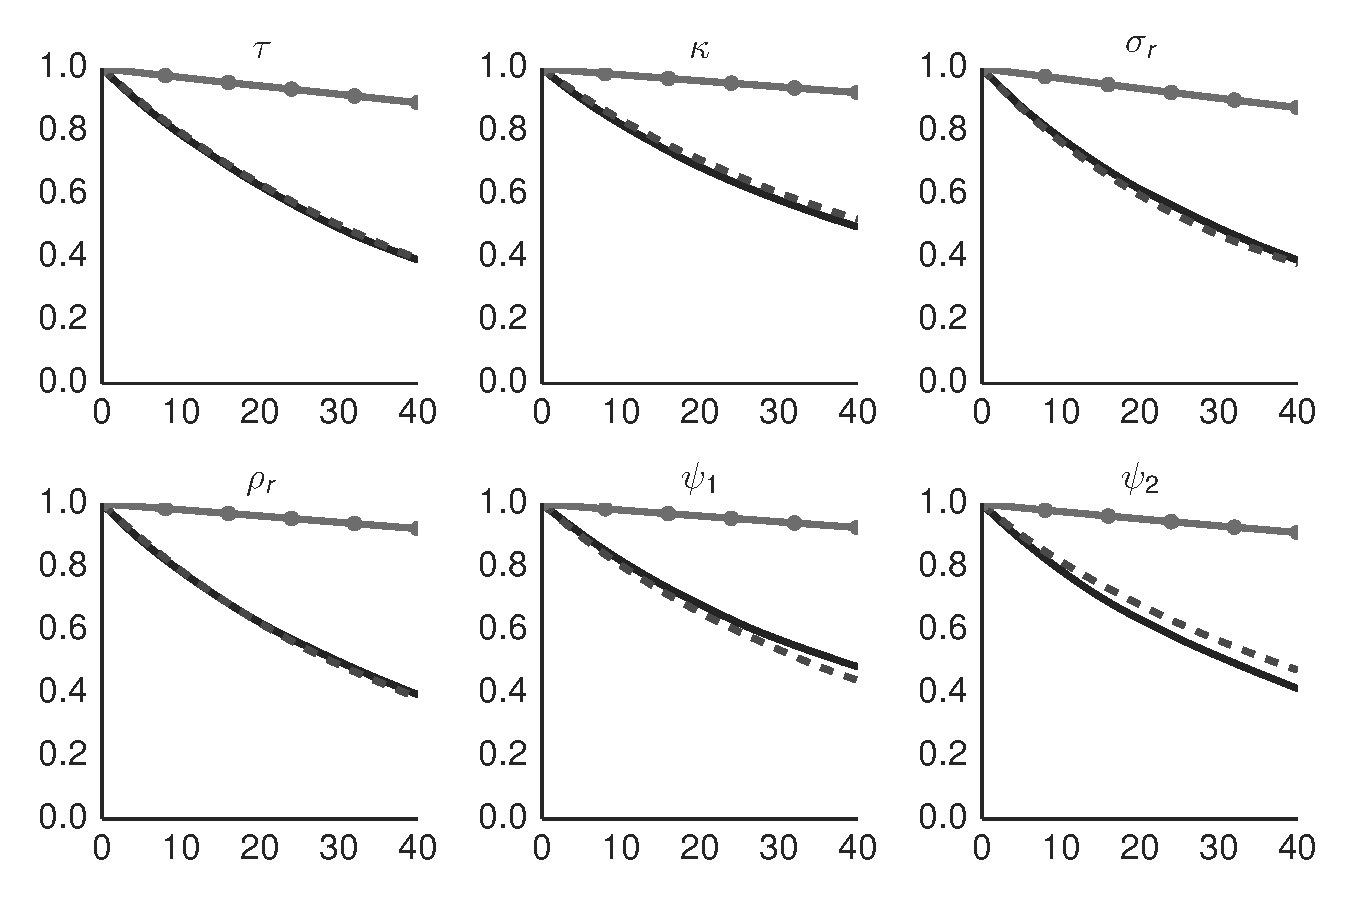
\includegraphics[width=3in]{dsge1_me_pmcmc_acf.pdf}
\end{center}
\emph{Notes}: The figure depicts autocorrelation functions computed from the
output of the 1 Block RWMH-V algorithm based on the Kalman filter (solid), the conditionally-optimal
particle filter (dashed) and the bootstrap particle filter (solid with dots).
\end{frame}



\begin{frame}[label={sec:org41839d3}]{Small-Scale DSGE: Accuracy of MH Approximations}
\begin{center}
	\scalebox{0.75}{
		\begin{tabular}{lccccccccc} \hline \hline
			& \multicolumn{3}{c}{Posterior Mean (Pooled)} & \multicolumn{3}{c}{Inefficiency Factors} & \multicolumn{3}{c}{Std Dev of Means} \\
			& KF    &  CO-PF&  BS-PF     & KF        &  CO-PF &  BS-PF     & KF        &  CO-PF &  BS-PF     \\ \hline
			$\tau$             &   2.63 &  2.62 &  2.64  &    66.17 &  126.76 & 1360.22  &  0.020 & 0.028 & 0.091 \\
			$\kappa$           &   0.82 &  0.81 &  0.82  &   128.00 &   97.11 & 1887.37  &  0.007 & 0.006 & 0.026 \\
			$\psi_1$           &   1.88 &  1.88 &  1.87  &   113.46 &  159.53 &  749.22  &  0.011 & 0.013 & 0.029 \\
			$\psi_2$           &   0.64 &  0.64 &  0.63  &    61.28 &   56.10 &  681.85  &  0.011 & 0.010 & 0.036 \\
			$\rho_r$           &   0.75 &  0.75 &  0.75  &   108.46 &  134.01 & 1535.34  &  0.002 & 0.002 & 0.007 \\
			$\rho_g$           &   0.98 &  0.98 &  0.98  &    94.10 &   88.48 & 1613.77  &  0.001 & 0.001 & 0.002 \\
			$\rho_z$           &   0.88 &  0.88 &  0.88  &   124.24 &  118.74 & 1518.66  &  0.001 & 0.001 & 0.005 \\
			$r^{(A)}$          &   0.44 &  0.44 &  0.44  &   148.46 &  151.81 & 1115.74  &  0.016 & 0.016 & 0.044 \\
			$\pi^{(A)}$        &   3.32 &  3.33 &  3.32  &   152.08 &  141.62 & 1057.90  &  0.017 & 0.016 & 0.045 \\
			$\gamma^{(Q)}$     &   0.59 &  0.59 &  0.59  &   106.68 &  142.37 &  899.34  &  0.006 & 0.007 & 0.018 \\
			$\sigma_r$         &   0.24 &  0.24 &  0.24  &    35.21 &  179.15 & 1105.99  &  0.001 & 0.002 & 0.004 \\
			$\sigma_g$         &   0.68 &  0.68 &  0.67  &    98.22 &   64.18 & 1490.81  &  0.003 & 0.002 & 0.011 \\
			$\sigma_z$         &   0.32 &  0.32 &  0.32  &    84.77 &   61.55 &  575.90  &  0.001 & 0.001 & 0.003 \\
			$\ln \hat p(Y)$ &    -357.14 & -357.17 & -358.32  & & & & 0.040 & 0.038 & 0.949 \\ \hline
		\end{tabular}
	}
\end{center}
\end{frame}


\begin{frame}[label={sec:org0c70297}]{Computational Considerations}
\begin{itemize}
\item We implement the PFMH algorithm on a single machine, utilizing up to
twelve cores.
\\~\\~
\item For the small-scale DSGE model it takes	 30:20:33 [hh:mm:ss]
hours to generate 100,000 parameter draws using the bootstrap PF with
40,000 particles.  Under the conditionally-optimal filter we only use
400 particles, which reduces the run time to 00:39:20 minutes.
\end{itemize}
\end{frame}




\section{Bibliography}
\label{sec:org30490b9}
\begin{frame}[fragile,allowframebreaks,label=]{References}
\bibliographystyle{apalike}
\bibliography{../../../../ref/ref}
\end{frame}
\end{document}